\Ax{

\begin{onecolumnfigure}[t]

\begin{fitheight}{3.2\standardhexwidth}
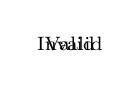
\begin{tikzpicture}
    \setfiguresize{-2.5}{-1.6}{+2.5}{+1.6}
    \drawevenhexgrid{-2}{-1}{5}{3}
    \drawcounter{-1.00}{-0.50}{45}{}{}{}
    \drawcounter{+1.50}{+0.75}{120}{}{}{}
    \drawcounter{+1.00}{+0.00}{45}{}{}{}
    \miniathex{-2.00}{+0.00}{\node {\scriptsize Valid};}
    \miniathex{+2.00}{+0.00}{\node {\scriptsize Invalid};}
\end{tikzpicture}
\end{fitheight}


\figurecaption{figure:ground-unit-map-location}{\protect\x{Map Location.}{Ground and naval units must be located in hexes; they may not be located on hex sides. Facing is only relevant for heavy AAA units and large naval units. The unit on the left has a valid location. The units on the right have invalid locations.}}

\end{onecolumnfigure}

}


